\documentclass[tikz, margin=10mm]{standalone}

\usepackage{tikz}

\usetikzlibrary{calc}
\usetikzlibrary{arrows, arrows.meta}

\begin{document}

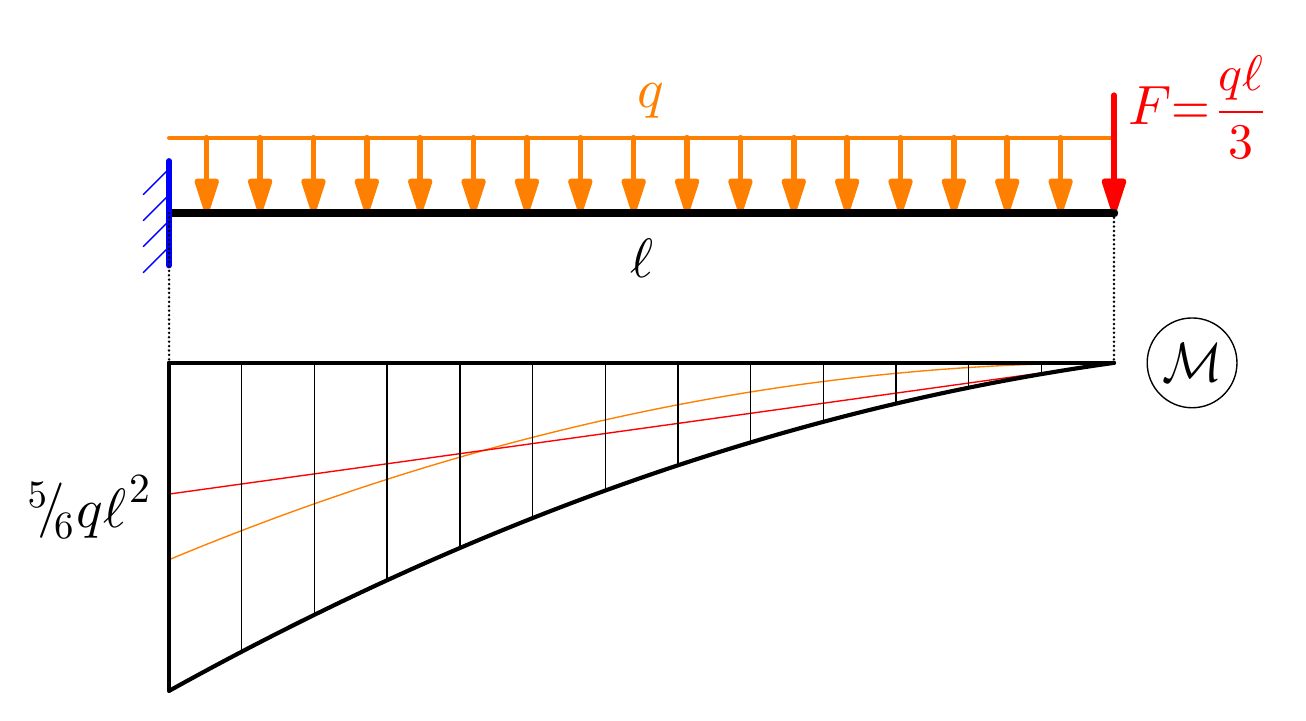
\begin{tikzpicture}[scale=1]

\def\beamlength{12}
\pgfmathsetmacro\halfbeamlength{\beamlength / 2}

% beam

%%\newcommand{\halfell}{ \raisebox{.3em}{$\ell$} \hspace{-0.4ex} / \hspace{-0.4ex} \raisebox{-0.33em}{\scalebox{0.88}{$2$}} }

\draw [line width=3pt, line cap=round, color=black]
	(0, 0) -- (\beamlength, 0)
		node [pos=0.5, below, shape=circle, fill=white, inner sep=-2pt, outer sep=11pt] {\scalebox{2}{$ \ell $}} ;

% external loads

\def\continuousloadheight{.96}
\tikzstyle{continuous load line} =
	[line width=2pt, orange, line cap=round, -{Triangle[round, length=15pt, width=9pt]}]
\tikzstyle{continuous load level} =
	[line width=1.5pt, orange, line cap=round]

\def\concentratedloadheight{1.5}
\tikzstyle{concentrated load line} =
	[line width=2pt, red, line cap=round, -{Triangle[round, length=15pt, width=9pt]}]

\pgfmathsetmacro\continuousstep{( \halfbeamlength + 0.1 ) / 9}
\pgfmathsetmacro\nextxcontinuous{\beamlength - \continuousstep}
\foreach \xcontinuous in {\beamlength, \nextxcontinuous, ..., 0}
	\draw [continuous load line] (\xcontinuous, \continuousloadheight) -- (\xcontinuous, 0) ;

\draw [continuous load level] (\beamlength, \continuousloadheight) -- (0, \continuousloadheight)
	node [pos=0.49, above, shape=circle, fill=white, inner sep=-2pt, outer sep=8pt] {\scalebox{2}{$q$}} ;

\draw [concentrated load line] (\beamlength, \concentratedloadheight) -- (\beamlength, 0)
	node [pos=0.1, right, shape=circle, fill=white, inner sep=-2pt, outer sep=2pt] {\scalebox{2}{$F\scalebox{.9}[1]{$=$}\hspace{.1ex}\scalebox{0.9}{$\displaystyle\frac{q\ell}{3}$}$}} ;

% redraw beam

\draw [line width=3pt, line cap=round, color=black] (0, 0) -- (\beamlength, 0) ;

% constraints

\def\clamplength{1.33}

\tikzstyle{constraint line} = [line width=2pt, color=blue, line cap=round]
\tikzstyle{constraint hatch} = [line width=.5pt, blue]

\def\hatchsize{.33}

\draw [line width=0pt, draw=white, fill=white]
	(0, \clamplength / 2) rectangle ++(-\hatchsize, -\clamplength) ;

\draw [constraint line] (0, 0) -- (0, \clamplength / 2) ;
\draw [constraint line] (0, 0) -- (0, - \clamplength / 2) ;

\pgfmathsetmacro\hatchamplitude{( \clamplength / 2 ) - .1}
\pgfmathsetmacro\hatchstep{.33}
\pgfmathsetmacro\nexthatch{\hatchamplitude - \hatchstep}
\foreach \yclamp in {\hatchamplitude, \nexthatch, ..., -\hatchamplitude}
	\draw [constraint hatch] (0, \yclamp) -- (-\hatchsize, \yclamp - \hatchsize) ;

% epure of bending moments

\def\epurepos{-1.9}

\def\momentqll{5} % scale of forces and moments
\pgfmathsetmacro\justq{\momentqll / (\beamlength * \beamlength)}
\pgfmathsetmacro\forceF{\justq * \beamlength / 3}

\tikzstyle{epure line} = [line width=1.5pt, color=black, line cap=round]
\tikzstyle{epure hatch} = [line width=.5pt, color=black]
\tikzstyle{epure aux} = [line width=1pt, color=black, line cap=round, dash pattern=on 0pt off 1.6\pgflinewidth]

\draw [epure aux] (0, 0) -- (0, \epurepos) ;
\draw [epure aux] (\beamlength, 0) -- (\beamlength, \epurepos) ;

\newcommand\momentfromq[1]{ ( \justq * #1 * #1 / 2 ) }
\newcommand\momentfromF[1]{ ( \forceF * #1 ) }
\newcommand\momentfunction[1]{ \momentfromq{#1} + \momentfromF{#1} }

\begin{scope}[shift={(\beamlength, \epurepos)}]
\draw [line width=.5pt, color=orange]
	plot [variable=\z, samples=100, domain=0:-\beamlength]
		(\z, - { \momentfromq{\z} }) ;
\draw [line width=.5pt, color=red]
	plot [variable=\z, samples=100, domain=0:\beamlength]
		(-\z, - { \momentfromF{\z} }) ;
\draw [epure line]
	plot [variable=\z, samples=100, domain=0:-\beamlength]
		(\z, - { \momentfunction{\z} }) ;
\end{scope}

\pgfmathsetmacro\epurehatchstep{\beamlength / 13}

\pgfmathsetmacro\nextxhatch{\beamlength - \epurehatchstep}
\foreach \xhatch in {\beamlength, \nextxhatch, ..., 0}
	\pgfmathsetmacro\righttoleftx{\beamlength - \xhatch}
	\pgfmathsetmacro\currentmoment{\momentfunction{\righttoleftx}}
	\draw [epure hatch] (\xhatch, \epurepos) -- (\xhatch, \epurepos - \currentmoment) ;

\draw [epure line] (0, \epurepos) -- (\beamlength, \epurepos) ;

\pgfmathsetmacro\endmoment{\momentfunction{\beamlength}}
\draw [epure line] (0, \epurepos) -- ++(0, -\endmoment) ;

% text

\newcommand\verynicefrac[2]{\raisebox{.11ex}{$ \raisebox{.3em}{\scalebox{0.7}{$#1$}} \hspace{-0.4ex} / \hspace{-0.46ex} \raisebox{-0.25em}{\scalebox{0.7}{$#2$}}\hspace{.15ex} $}}

\newcommand\ellsquared{ \ell^{\hspace{.1ex}\scalebox{.75}{\raisebox{.1em}{$2$}}} }

\newcommand\internalmoment{\scalebox{.9}[1]{$ \mathcal{M} $}}

\draw [epure aux] (0, \epurepos) -- (0, \epurepos - \endmoment)
	node [pos=0.44, left, shape=circle, fill=white, inner sep=-2pt, outer sep=6pt]
	{\scalebox{2}{$ \verynicefrac{5}{6} q \ellsquared $}} ;

\node [right, shape=circle, draw=black, line width=.5pt, fill=white, inner sep=2.5pt, outer sep=12pt]
	at (\beamlength, \epurepos) {\scalebox{2}{$ \internalmoment $}} ;

\end{tikzpicture}

\end{document}